% !TeX root = ../thesis.tex

\begin{savequote}[75mm]
The most exciting phrase to hear in science, the one that heralds new discoveries, is not 'Eureka!' but 'That's funny...'
\qauthor{Isaac Asimov}
\end{savequote}
\chapter{State of the art} \label{chap:sota}


In this chapter, we cover some fundamental concepts and connections between some of the most important fields of study that are relevant to this thesis. We will start by covering the basics of \ac{ai} and its history and how it came to be the powerhouse and almost generic term that it is today. Then we will follow up to \ac{ebm} and its importance to modern medicine, some barriers and benefits of following such practice and paradigm. Thirdly, we will focus on \ac{kdd} and how healthcare databases can provide support for new knowledge.

Then we will cover the field of \ac{heads} and its connections to \ac{ai}, \ac{ebm} and \ac{kdd} as a way of bringing all of these together. We will then cover the field of \ac{xai} and its connections and \ac{cml} and how these subfields are vital to tackle modern medicine and a cornerstone of building trust in computerized systems and autonomous decision support tools. We conclude this chapter by covering some legal and ethical considerations relevant to this thesis.


\section{Artificial Intelligence}
% !TeX root = ../thesis.tex

\ac{ai} has already been under public focus for a few years now, but its concept is still elusive, mainly because the definition has been changing rapidly as well.
From the very beginning, the field of \ac{ai} focused not only on understanding but also on building intelligent entities \cite{DBLP:books/aw/RN2020}. Intelligent entities can be understood as machines that can act according to what is expected in a wide range of situations.
The first work of \ac{ai} could be credited to Warren McCulloch and Walter Pitts (1943) with the proposed model of artificial neurons. In the 50s, \ac{ai} could be associated with the works of Christopher Strachey, of two chess-playing programs.
In the 60s, the perceptrons could be indicated as state-of-the-art \ac{ai}. In the 80s, expert systems provided advanced reasoning with which the so-called weak methods of previous iterations could not compete.
The 90s brought the probabilistic reasoning and \ac{ml} which led to more robust systems that went further than the boolean logic used so far. In the 2000s, big data and \ac{ml} got focused on. Big data was used as a matter symbolizing the increasing amounts of data in some industries \cite{dashBigDataHealthcare2019}, and \ac{ml} as \textit{ the study of computer algorithms that improve automatically through experience} \cite{mitchell1997machine}. This last definition is especially important since it is currently used as a synonym of \ac{ai} across several industries but have actual different meanings as discussed below. This era probably peaked around the IBM Watson victory in jeopardy, but with way fewer interesting results in healthcare \cite{swetlitzIBMWatsonSupercomputer2018}, and 2010s brought deep learning. 
Nowadays, \ac{ai} is a buzzword that is used to describe a wide range of systems, from the simplest to the most complex. It is clearly trending, reports on \ac{ai} show that papers regarding the subject have seen a 20-fold increase from 2010-2019.
%cite (20fold)
To define \ac{ai}, we can refer to the description given by a team of specialists whom the European Commission tasked with developing guidelines on \ac{ai} \cite{DefinitionAIMain2019}. This document clarifies that initially, it is essential to distinguish between intelligence and rationality. Intelligence, being more subjective and philosophical, differs from rationality, which is pragmatic and linked to the ability to select the optimal course of action in a given situation to achieve a specific goal. While rationality is a more tangible concept and not identical to intelligence, it should be considered an integral component of it \cite{DefinitionAIMain2019,DBLP:books/aw/RN2020}.
From these two concepts, we can go even deeper, and define that rationality can be achieved in an \ac{ai} system by perceiving the environment, reasoning with what is perceived, and acting on the environment. From these three elements, we can argue that reasoning is the core functionality, which is related to taking data, understanding it or interpreting it, and reasoning on this data through a model (numerical or symbolical) to reach the best action.

There is also the need to address the current distinction for \ac{ai} which is the narrow and general \ac{ai}. The first is the one that exists nowadays and it's an \ac{ai} that is not generic, it is focused on a specific task. The second is the one that is not yet achieved, and it is the one that is more generic and can be applied to several tasks. This is the one that is usually associated with the popular or common concept of \ac{ai} \cite{DefinitionAIMain2019,DBLP:books/aw/RN2020}. So, with this is mind, \ac{ai} can be defined as:
\begin{quote}
    \textit{Artificial intelligence systems are software (and possibly also hardware) systems designed by humans that, given a complex goal, act in the physical or digital dimension by perceiving their environment through data acquisition, interpreting the collected structured or unstructured data, reasoning on the knowledge, or processing the information, derived from this data and deciding the best action(s) to take to achieve the given goal. \ac{ai} systems can either use symbolic rules or learn a numeric model, and they can also adapt their behaviour by analysing how the environment is affected by their previous actions. As a scientific discipline, \ac{ai} includes several approaches and techniques, such as machine learning (of which deep learning and reinforcement learning are specific examples), machine reasoning (which includes planning, scheduling, knowledge representation and reasoning, search, and optimization), and robotics (which includes control, perception, sensors and actuators, as well as the integration of all other techniques into cyber-physical systems).} \cite{DefinitionAIMain2019}
    \end{quote}
    
Certainly, given the rapid advancements in this field, this concept might become outdated swiftly. Nonetheless, it serves as an effective starting point for grasping the fundamentals of \ac{ai} and its implications.

%This is connected with the concept that \ac{ai} is tightly connected with the subjective nature of humans. If we feel that \ac{ai} is something related to what a human can do, it can be widely diverse from person to person.

%however, there are some definitions that could be interesting to explore in order to get the concept for the purpose of this thesis cleared up.



\section{Evidence Based Medicine}\label{subsec:ebm}

In 1996, David Sacket and colleagues defined \ac{ebm} as \textit{the conscientious, explicit, and judicious use of current best evidence in making decisions about the care of individual patients} \cite{sackettEvidenceBasedMedicine1996}. Despite having historical antecedents dating back to at least the 19th century, the first time the term "evidence-based medicine" was first coined by a team at McMaster University in Canada in the 1980s \cite{thomaBriefHistoryEvidenceBased2015}. This was a time when clinical decision-making was mostly based on untested observations and physicians' experience, leading to variability in treatment strategies. The birth of \ac{ebm} marked a pivotal moment in medical history, aiming to standardize patient care and improve outcomes. So, \ac{ebm} is still a relatively recent concept in healthcare, which entails integrating the best available research evidence with clinical experience and patient values to make decisions about patient care. 
With this, we can, as stated by Sacket, define \ac{ebm} into 3 major pillars:
\begin{myitemize}
    \item Best available evidence
    \item Clinical expertise
    \item Patient values, expectations, and/or wishes.
\end{myitemize}

Clinical expertise refers to the acumen and discernment gained from hands-on clinical experiences and consistent practice. This expertise manifests notably in enhanced diagnostic abilities and in the considerate recognition of a patient's unique circumstances, rights, and wishes when making care decisions. The term 'Best available evidence' pertains to pertinent clinical studies, often stemming from epidemiological investigations. This is linked with the ability (and willingness) to challenge current diagnostic methods and treatments, introducing alternatives that are more robust, precise, effective, and safer. 
Without experience, clinical practices blindly follow the best available evidence, which is not always the best option for the patient, since sometimes it may be inapplicable to a specific scenario. Without evidence, clinical practice becomes stagnated and unable to evolve \cite{sackettEvidenceBasedMedicine1996}.


The main concept of \ac{ebm} is the hierarchy of evidence, which classifies different types of research studies based on their methodological quality and applicability to patients. At the top of this hierarchy are \acp{rct} and systematic reviews of \acp{rct}, which are considered to provide the most robust evidence. Observational studies, case series, and expert opinions are further down the hierarchy due to their inherent limitations (figure \ref{fig:ebm}). \ac{ebm} advocates for the application of the highest level of evidence available in clinical decision-making.
\begin{figure}
    \centering
    %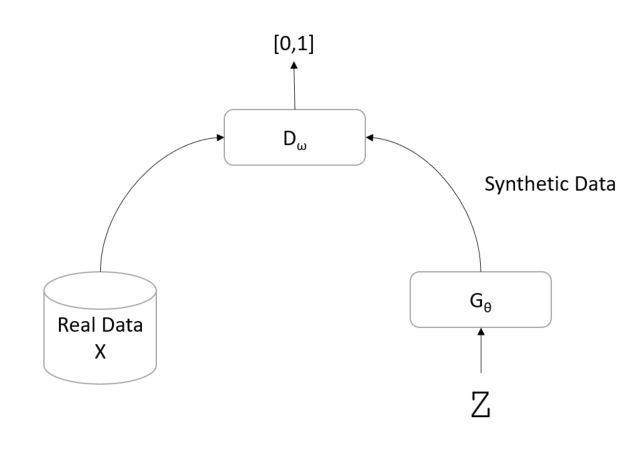
\includegraphics[width=\textwidth]{image.png}
    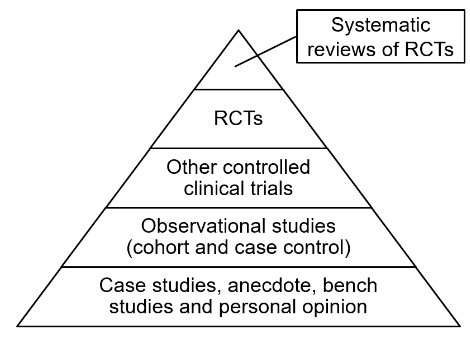
\includegraphics[scale=0.55]{figures/ebm.png}
    
    \caption{\acl{ebm} diagram adapted from \cite{greenhalghHowReadPaper2019}} \label{fig:ebm}
    \end{figure}

Historically, medical decisions leaned heavily on anecdotal observations and the prevailing beliefs of seasoned practitioners. To underscore the dangers of relying solely on such expert opinions, Sackett frequently recounted the circumstances surrounding George Washington's unfortunate end. Despite being in good health at the age of 68, Washington developed epiglottitis. Rather than opting for a tracheostomy, a treatment method known since ancient Greek times, his physicians, guided by the prevailing expert opinion, chose bloodletting as the course of action. Tragically, this decision led to Washington's likely preventable death, highlighting the critical importance of grounding medical decisions in robust evidence.
However, \ac{ebm} is not without critiques. The first one is that this is what medicine is all about and is already practiced all over. The data suggest something different \cite{sackettEvidenceBasedMedicine1996}.
The second refers to the virtually impossible task of keeping up with the literature. This argument, despite being refuted by examples of clinicians doing it, does raise the question of how we can deal with this, taking into account the increasing evidence overflow that the current times bring. How can we keep up with the literature and how can we make sure that the evidence is being applied in clinical practice? This is a very important question since the evidence is only useful if it is applied. This is where \ac{kdd} and \ac{ai} can play a role, as we will see in the next sections. 





\section{Extracting Knowledge from Data}\label{sec:kdd}
%%%TODO: explorar mais artigos recolhidos e ver zotero o que ja tenho, e criar mais ligacoes entre as frases e conceitos
% !TeX root = ../thesis.tex

%fayyad explorar mais e melhor intro
\ac{kdd} is about turning data into knowledge. However, turning data into knowledge or insights is not new in healthcare. The first attempts to use data to improve healthcare date back to the 17th century, when John Graunt used data from the London Bills of Mortality to study the causes of death in the city \cite{741e4dcd-5d3c-325c-9241-5eb5ddd0cb60}. This was the first time that data were used to understand the health of a population. Since then, the field of \ac{kdd} has evolved significantly, and it is now a crucial part of healthcare, helping to improve patient outcomes, enhance clinical decision-making, and optimize healthcare delivery.

Additionally, the fact that data are being collected at an unprecedented rate, and the need to extract knowledge from them, has led to the development of several methodologies and frameworks to map low-level data (granular) into short reports, more abstract, or more useful formats \cite{Fayyad_Piatetsky-Shapiro_Smyth_1996}. So, it is only natural to see that \ac{kdd} has become very popular in a wide range of industries nowadays.

Healthcare is no exception, and \ac{kdd} has been applied to several areas of healthcare, from clinical decision support to disease surveillance and outbreak detection. Reports and papers suggest that \cite{dashBigDataHealthcare2019} the digital data in the healthcare space have been increasing rapidly, due to the adoption of \ac{ehr} and similar digital tools in the healthcare space. 

The complexity and vastness of healthcare data, encompassing electronic health records, genomic data, medical imaging data, and various other types of data, call for the adoption of intelligent systems that can mine this data for useful insights. The \ac{kdd} process, comprising data cleaning, integration, selection, transformation, data mining, pattern evaluation, and knowledge presentation, can effectively help discover patterns and relationships in healthcare data, which are often not apparent to traditional analysis methods. This process facilitates the prediction of disease outbreaks, the identification of high-risk patient groups, the optimization of treatment plans, and the enhancement of healthcare service delivery. The generic process for \ac{kdd} is shown in figure \ref{fig:kdd-generic}.

\begin{figure}
\centering
%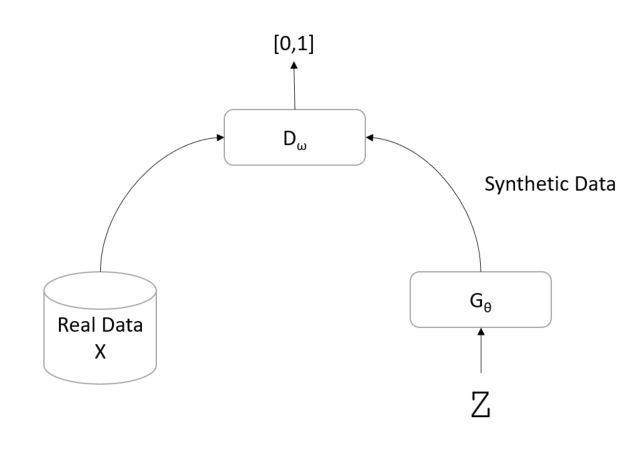
\includegraphics[width=\textwidth]{image.png}
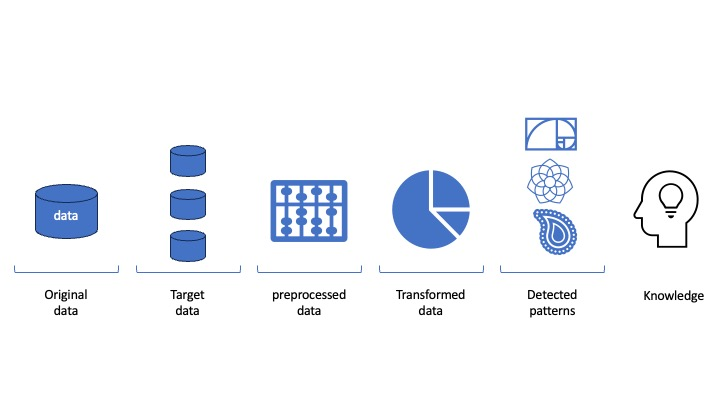
\includegraphics[scale=0.55]{figures/imagens-tese.jpg}

\caption{\acl{kdd} Process, adapted from \cite{Fayyad_Piatetsky-Shapiro_Smyth_1996}} \label{fig:kdd-generic}
\end{figure}

Several frameworks have been proposed to implement the \ac{kdd} process. One such prominent framework is \ac{crispdm}, which comprises business understanding, data understanding, data preparation, modelling, evaluation, and deployment. \ac{crispdm} was conceived in 1996 and became a \ac{eu} project under the ESPRIT funding initiative in 1997 \cite{Chapman2000CRISPDM1S}. \ac{semma} \cite{rohanizadehProposedDataMining2009} involves five stages: sampling, exploration, modification, modelling, and assessment. It starts by analyzing a subset of data, then seeks patterns and modifies variables. A model is built, and the results are evaluated. While \ac{semma} covers key data-mining aspects, it misses fundamental components of information system projects like analysis and implementation.

It is important to distinguish, however, that \ac{kdd} is not the same as Data Mining. As stated in \cite{Fayyad_Piatetsky-Shapiro_Smyth_1996}, we agree that \ac{kdd} is a major process of which Data Mining is a part. So, in order to understand the process of \ac{kdd}, we need to understand the process of Data Mining, which can be understood as the application of algorithms for extracting patterns from data. There are several classes of algorithms, each best suited for different kinds of tasks:
\begin{itemize}
    \item Classification Algorithms: These are used to predict categorical class labels. Examples include Decision Trees, Naive Bayes, \ac{svm}, \ac{knn}, and various types of Neural Networks. These are used in disease diagnosis, patient risk prediction, and readmission prediction.
    \item Clustering Algorithms: These are unsupervised methods used to group similar data points together. K-Means, Hierarchical Clustering, DBSCAN, and Self-Organizing Maps are common clustering algorithms used in patient segmentation and anomaly detection.
    \item Regression Algorithms: These are used to predict continuous output variables. Examples include Linear Regression, Logistic Regression, and Regression Trees. These algorithms find application in predicting disease progression and healthcare costs.
    \item Association Rule Mining Algorithms: These discover associations or patterns among a set of items in large databases. \textit{Apriori} and FP-Growth are commonly used algorithms in this class, helping in discovering co-occurring health conditions or drug interactions.
    \item Sequential Pattern Mining Algorithms: These help discover or predict specific sequences of events, which is particularly useful in medical trajectory analysis.
    \item More sophisticated architectures and algorithms appeared with neural networks, generative \ac{ai}, and reinforcement learning, among others.
\end{itemize}

As a result, \ac{kdd} is the process of applying Data Mining algorithms to data but also the data preparation, selection, cleaning, and most important of all, the incorporation of prior knowledge about the domain along with the proper interpretation of results. This difference is vital to understanding \ac{kdd}, since blindly applying data mining or \ac{ml} methods to data will only render results that are not useful or even misleading \cite{Fayyad_Piatetsky-Shapiro_Smyth_1996}.

In short, \ac{kdd} can be understood as a multidisciplinary subject that bridges and aggregates knowledge from different areas like \ac{ml}, pattern recognition, databases, statistics, \ac{ai}, knowledge acquisition for expert systems, data visualization, and high-performance computing. On top of all of these subjects and research areas sits the most important of all—which is domain expertise.

%-tipos de algortimos paraa




\section{Health Data Science}

% !TeX root = ../thesis.tex

%sacket 
%graph of evidence based medicine
%inconvenient truth ai
%Three controversies in \ac{heads}
\ac{heads} is an interdisciplinary field that applies rigorous methods to transform healthcare data into actionable knowledge for improving health outcomes. It involves the collection, interpretation, and application of vast amounts of biological, clinical, population, and health system data to improve patient care and public health. The advent of electronic health records, genomics, mobile health technologies, and other forms of big data have fuelled the growth of this discipline.

In practice, \ac{heads} involves the use of statistical and machine learning methods to analyse healthcare data. This data can be patient records, genomic data, demographic data, and more. It includes elements from various disciplines like biostatistics, epidemiology, informatics, and health economics. The ultimate goal is to provide a data-driven foundation for health decision-making for clinicians, health administrators, policymakers, and researchers.

An integral part of \ac{heads} is predictive modelling and hypothesis testing. Predictive modelling involves the creation and use of statistical models or machine learning algorithms to predict future outcomes based on historical data. Hypothesis testing, on the other hand, is used to test the validity of a claim or theory about a population based on sample data. These are crucial for \ac{heads} as they allow us to make educated guesses about health trends and outcomes.

Importantly, \ac{heads} has significant ethical and privacy considerations. Health data is often sensitive and personal, so maintaining privacy and confidentiality is crucial. This requires secure data handling and storage practices, as well as careful consideration of ethical implications when designing studies and algorithms. Health Data Scientists must also be wary of algorithmic bias and must ensure their models do not perpetuate or amplify health disparities. The ultimate goal of \ac{heads} is to improve patient outcomes and health equity using the best available data and methods.


The potential of using systematically created data in healthcare has certainly a lot of potential. However, we have seen in the past as well, that the hype of \ac{ai} and \ac{ml} usually are not supported by truth. There are currently six main aspects that hinder the potential of \ac{heads} \cite{panchInconvenientTruthAI2019,peekThreeControversiesHealth2018}:
\begin{myitemize}
    \item Interoperability
    \item Semantic
    \item Secondary usage
    \item Data quality
    \item Privacy and ethics
    \item Observational data
\end{myitemize}

\textbf{Interoperability} is defined by \textit{the ability of two or more systems or components to exchange information and to use the information that has been exchanged} \cite{182763}. In the context of healthcare, this means that different systems should be able to exchange data and interpret the data that has been exchanged. This is a very important aspect of \ac{heads} since the data is usually stored in different systems, with different structures and different purposes. So, if systems are locked inside themselves and no export is possible, data becomes inaccessible. So, it is only natural that interoperability has been a key factor in gathering data. With tens or hundreds of different systems in every health institution, the possibility of exchanging data between \acp{ehr} plays a vital role. The usage of interoperable standards is of extreme importance in order to tackle the need to get data with a predefined structure.


\textbf{Semantic} adds a layer to the previous points, being sometimes related to interoperability as well. The fact that several institutions and \acp{ehr} are involved in creating knowledge from data, raises the problem that not all have data coded in clinical terminologies, or if they do, it is seldom the same across systems, since semantics has a very tight relationship with domain, especially in healthcare. So the normalization of uncoded terms is often required and mapping across terminologies is also very common, which is time-consuming and requires expertise in several fields.



%mts ehrs
%mts 
\textbf{Secondary usage} is related to the fact that we are aiming to use data for a purpose for which the data was not created. The main goal of the healthcare data is to provide care. It is not meant for analysis and gaining insights. More than that, is already pretty well documented that the usage of \ac{ehr} is very different from institution to institution and from country to country \cite{anckerHowElectronicHealth2014,weiskopfMethodsDimensionsElectronic2013a,peekThreeControversiesHealth2018}. This means that the context where data was collected, even the actual person who inserted the information could be key to interpreting the results. To make things more complicated, the degree of precision of the data inserted varies highly on the type of information and context, as reported in \cite{cruz-correiaDataQualityIntegration2009}. 



\textbf{Data Quality} stems from the secondary usage. If the data is not reliable, how can we use it to gather useful knowledge from it? In order to, at least, try to counter this, we can apply several statistical methods and machine learning algorithms to try to clean the data. However, this is not a trivial task, since the data is usually very heterogeneous and the context where it was collected is not always available. So, data quality is a very important aspect of \ac{heads}, since it can be the difference between a good and a bad model.



\textbf{Privacy and ethics} add yet another layer to the problems of \ac{heads}. The fact that we are dealing with sensitive private data, which is not meant to be used for secondary purposes, raises the question of privacy and ethical concerns. Anonymization techniques and privacy-preserving methods are key to tackling this problem. However, they are not problem-free and are often complicated to assess. Moreover, the risks are very high, since the data is very sensitive and the consequences of a breach of privacy can be very serious, undermining public trust in clinicians, healthcare institutions and the healthcare system as a whole.

%%%LLM
%\ac{heads} and evidence-based medicine are closely intertwined fields that leverage the power of data analysis and research to improve patient outcomes and inform clinical decision-making. \ac{heads} involves the collection, management, and analysis of vast amounts of health-related data, including electronic health records, medical imaging, genomics, and wearable devices. By applying advanced statistical and machine learning techniques to these datasets, health data scientists can uncover patterns, trends, and insights that can enhance our understanding of diseases, treatment effectiveness, and population health.

%Evidence-based medicine, on the other hand, is an approach to clinical practice that integrates the best available research evidence, clinical expertise, and patient values and preferences. It aims to guide healthcare professionals in making informed decisions about patient care by using rigorous scientific evidence. \ac{heads} plays a crucial role in evidence-based medicine by providing the necessary data and analytical tools to generate high-quality evidence. Through the analysis of large-scale health datasets, researchers can identify associations, evaluate treatment effectiveness, and uncover potential risk factors, all of which contribute to the evidence base that informs clinical practice guidelines and treatment recommendations.
\textbf{Observational Data} relates to the fact that all \ac{heads} will be based on observational data. This means that the data is not collected in a controlled environment, which is the case for \acp{rct}. Consequently, this data is subject to several biases, which are not always possible to control. The cornerstone of \acp{rct} is simply not possible to apply here, preventing a proper comparison between groups. Even though there are techniques to tackle the unbalance in the measured variables, there is no way to control the unmeasured variables, which can be the cause of the observed effect. This is of particular importance and a major area of research at the moment, as we will see in the sections \ref{subsec:xai} and \ref{causalml}.

With this in mind, it is natural to assume that \ac{heads} and \ac{ebm} are very synergic. If, on the one hand, we could argue that \ac{kdd} can take \ac{ebm} even further by using Data Mining and \ac{ai} to produce synthetic evidence by analysing, summarizing, or even combining evidence from several sources in order to feed medical practice with the best evidence available in a useful manner. On the other hand, we could also argue that \ac{ebm} can be used to guide the \ac{kdd} process, by providing the necessary domain knowledge to interpret the results and to guide the process of data preparation, selection, and contextualization. The domain knowledge mentioned in the \ac{kdd} section could be applied by \ac{ebm}.

The synergy of \ac{kdd} and \ac{ebm} has the potential to revolutionize healthcare delivery and improve patient outcomes. By leveraging the power of data analysis and advanced algorithms, health data scientists can identify novel biomarkers, develop predictive models, and personalize treatment plans based on individual patient characteristics. This not only enhances clinical decision-making but also enables precision medicine, where treatments can be tailored to the specific needs of each patient. Additionally, the use of \ac{heads} in evidence-based medicine allows for the continuous monitoring of treatment effectiveness and safety, facilitating the identification of best practices and the refinement of clinical guidelines over time.


\section{Explainable Artificial Intelligence}\label{subsec:xai}

\ac{ai} has experienced unprecedented advancements in the last decade, leading to its integration in various domains, including medicine. It has been instrumental in transforming clinical decision-making, drug discovery, patient monitoring, and predicting disease trajectories. Despite these advancements, the "black box" nature of complex \ac{ai} models poses interpretability challenges, limiting their widespread adoption in healthcare, a field where transparency, reliability, and understanding of decision-making processes are vital. This lack of interpretability, also known as opacity, can lead to misdiagnoses, inappropriate treatment plans, and, most importantly, breaches in trust among clinicians, patients, and \ac{ai} systems.

As such, the concept of \ac{xai}, which aims to create a suite of techniques that produce more explainable models while maintaining a high level of predictive accuracy, has gained significant attention in medical \ac{ai} research. \ac{xai} seeks to bridge the gap between \ac{ai} opacity and human interpretability, and in doing so, it can enhance the transparency, reliability, and acceptance of \ac{ai} applications in the healthcare setting.

So, for this to happen, we need a new framework for applying such mechanisms. A new step that could be attached to the ones seen before in section \ref{sec:kdd} will enable human comprehension of the model's output.

Even though several grouping and taxonomies of \ac{xai} are available mentioned in \cite{adadiPeekingBlackBoxSurvey2018,linardatosExplainableAIReview2020,barredoarrietaExplainableArtificialIntelligence2020,linardatosExplainableAIReview2020,kamath2021explainable}, a simplified approach based on \cite{kamath2021explainable} will be used in order to contextualize this concept.

We can divide it into two main categories. Firstly, the explanation type is divided into global and local. Local and global explanations are methods used to interpret machine learning models, especially those that are considered "black box" models, such as deep learning networks. These methods help us understand why and how a model makes certain decisions, which can be crucial in many settings for ethical, legal, and practical reasons.

Local Explanations: These involve understanding the prediction of a \ac{ml} model for a specific individual instance. They help to answer questions like: "Why did the model predict that this particular patient has cancer?" or "Why was this specific transaction flagged as fraudulent?". 

Global Explanations: These focus on understanding the model behaviour across all instances, or more broadly on a dataset-wide level. They help to answer questions like: "What features are generally important for prediction in the model?" or "What is the overall logic of the model?". 

Secondly, we have the method type, where we have 3 main subcategories related to the stage of the data science process it is applied, \textit{pre}, during, and \textit{post}-model training.

\textbf{Pre-Model \ac{xai}:} These methods involve improving the transparency and interpretability of models before they are even trained. This includes thoughtful feature engineering, \ac{eda}, and applying domain knowledge to create meaningful variables. The goal is to design a model that will be more interpretable from the onset.

\textbf{Intrinsic \ac{xai}:} This involves using machine learning models that are intrinsically explainable. These models are designed in such a way that their decision-making process is understandable by default. Examples include linear and logistic regression, cox regressions, decision trees, Naïve Bayes, \ac{bn}, and rule-based models. While these models may sometimes lack the predictive power of more complex models, they provide clear interpretability: you can directly examine the impact of the variables and understand how the model makes its predictions.
\\
\textbf{Linear Regression} is a linear approach to modelling the relationship between a dependent variable and one or more independent variables. It assumes that the relationship between these variables is linear and can be represented by a straight line. The goal is to fit the best possible line that describes this relationship by minimizing the sum of the squared differences (errors) between the observed values and the values predicted by the line. Linear regression is widely used in various fields for prediction, modelling, and determining the strength and character of the relationship between variables. It forms the basis of many more complex statistical modelling techniques.
\\
\textbf{Logistic Regression} is used to model the probability of a binary outcome that depends on one or more independent variables. Unlike linear regression, which predicts a continuous outcome, logistic regression predicts the probability of a categorical outcome (e.g., success/failure, yes/no, 1/0). The logistic function is applied to the linear combination of independent variables to ensure that the estimated probabilities are between 0 and 1. It's often used in fields like medicine, economics, and social sciences to predict the likelihood of an event occurring based on various factors.
\\
\textbf{Cox Regression} or the Cox proportional-hazard's model, is a statistical technique used for investigating the effect of several variables on the time a specified event takes to happen. In medical research, this often refers to survival times. The model allows for the estimation of hazard ratios, which describe how the hazard changes with a one-unit change in the predictor variable. The Cox model makes an assumption that the hazard ratios are constant over time, known as the proportional hazard's assumption. This model is vital for understanding how different factors influence survival or failure time and is commonly applied in epidemiological and medical research.

\textbf{Bayesian Networks}
A \ac{bn}, also known as a belief network or \ac{dag} model, is a probabilistic graphical model that represents a set of random variables and their conditional dependencies via a \ac{dag}. 

Given a set of variables \(X = \{X_1, X_2, ..., X_n\}\), the joint probability distribution is given by:

\[
P(X_1, X_2, ..., X_n) = \prod_{i=1}^{n} P(X_i | Parents(X_i))
\]

where \(Parents(X_i)\) is the set of parent variables of \(X_i\) in the network.

This formula represents the factorization of the joint distribution over \(X\), based on the graphical structure of the Bayesian network.

Now, in the Bayesian network, each node is conditional independent of its non-descendants given its parents. If we denote \(ND(X_i)\) as the set of non-descendants of \(X_i\) and \(Pa(X_i)\) as the parents of \(X_i\), the conditional independence is described as:

\[
X_i \perp ND(X_i) | Pa(X_i)
\]

This means that \(X_i\) is conditionally independent of its non-descendants given its parents. 

A common task for Bayesian networks is inference, which means computing the posterior probability of a set of query variables \(Q\), given some observed variables \(E\). That is, we want to compute \(P(Q|E)\). According to the Bayes rule, we have:

\[
P(Q|E) = \frac{P(Q,E)}{P(E)} = \frac{P(Q,E)}{\sum_{q \in Q} P(Q=q,E)}
\]

where the denominator is a normalization constant ensuring the result is a valid probability distribution. Note that performing this inference is NP-hard, which is why various approximation algorithms have been developed.

\textbf{Tree based methods}
Tree-based machine learning methods are a subset of algorithms that use a tree-like graph structure for making decisions or predictions. The most basic type is the Decision Tree, where the tree is used to go from observations about an item to conclusions about the item's target value (classification or regression). Each node in the tree represents a feature in the dataset, each branch represents a decision rule, and each leaf node represents the output value. More advanced tree-based methods include Random Forests, which build multiple Decision Trees and average their predictions for better accuracy and generalization, and gradient-boosted trees, which build trees sequentially, each one correcting the errors from the previous one.

The major advantage of tree-based methods is their ease of interpretation and understanding, especially for Decision Trees. However, a single tree is often prone to overfitting, where it performs well on the training data but poorly on unseen data. This is why ensemble methods like Random Forest and Gradient Boosting are popular; they aim to increase robustness and predictive power by combining multiple trees. These methods are widely used in various domains including but not limited to finance, healthcare, and natural language processing for tasks like classification, regression, and even unsupervised learning tasks like clustering.

\textbf{Post-Hoc \ac{xai}:} Post-hoc methods are applied after a model has been trained, to try to explain its decisions. This includes techniques like feature importance analysis, partial dependence plots, \ac{lime}, \ac{shap}, and counterfactuals. For instance, \ac{lime} can be used to create local explanations for individual predictions made by any model, and \ac{shap} values can be used to interpret the impact of features on the model's output both locally and globally. Counterfactuals try to explain a model by example, providing possible changes that would alter the outcome provided by the model.

It is to be noted that a methodology can be classified into two categories. For example, \ac{lime} is a local explanation model in a \textit{post-hoc} manner.

Despite all of this, we  have to take into account that pre-model and post-hoc methodologies are a proxy for an explanation of the models. That is why we could argue, as stated in \cite{rudinStopExplainingBlack2019} that only an intrinsically transparent model can really be the basis of \ac{xai}. While \textit{post-hoc} of pre-model methods are only a potentially unreliable proxy for an explanation.
%explicar mais disto e fechar.



\section{Causality}\label{causalml}

% !TeX root = ../thesis.tex

Using, once again, the tale of George Washington but now with a different purpose; the medical doctors in that region of the globe, at least, followed the theory of humours, which relied on the fact that a healthy human person was a balance between four humours (blood, phlegm, yellow bile, and black bile). So, the treatment for George Washington was to rebalance those four humours, and so, doctors needed to remove blood, which was the supposed cause of his illness. Since microbiology and its importance would only be discovered sometime after, the idea at the time was inspired by the fact that the imbalance of these four senses of humour and illness was present at the same time.

This is now known as a textbook definition of confounding correlation with causation. And in this subject in particular, it was not the imbalance in the humours that caused illness, but an illness that caused the imbalance.

So, this example shows that evidence without proper causality can lead to misguided results and mistrust.

That is why, nowadays, \ac{ebm} and \ac{xai} can be brought together and expanded through \ac{cml}. But what is causality? We could argue that it is related to something \textbf{causing} something else. This causal effect, especially in medicine, can be related to a comparison of the outcome a particular person would exhibit given a particular intervention and the outcome in the same person of the control intervention. This is particularly hard since we cannot do both things at the same time. This is the basis of why \acp{rct} are the gold standard of experimentation, since they are the current best tool to achieve something similar to this \cite{10.7551/mitpress/14244.001.0001}.

%- causality vs observation

\ac{cml} is a branch of \ac{ml} that focuses on understanding and quantifying causal relationships from data \cite{hernanDefinitionCausalEffect2004}. Instead of just finding patterns or correlations in data, \ac{cml} aims to uncover the cause-and-effect relationships that explain these patterns.
This is especially important since current or traditional \ac{ml} and \ac{ai} methodologies rely heavily on association and not causation. So, \ac{cml} can support traditional algorithms to solve its limitations \cite{pearlTheoreticalImpedimentsMachine2018}.
There are currently two main frameworks for trying to unveil causality in data: the \ac{scm}  and the \ac{pof} \cite{shiLearningCausalEffects2022b}. \textbf{\ac{scm}} relies on 1) Causal Graphs and 2) structural equations.

\begin{enumerate}
    \item Causal Graphs are based on \acp{dag}: These are graphical models used to represent causal relationships between different variables. The nodes in the graph represent variables, and the edges (arrows) between nodes represent causal relationships. For instance, an edge from Node A to Node B signifies that A has a causal effect on B. We should not confuse causal graphs with \ac{bn}. Even though both rely on \acp{dag}, Causal Graphs represent causal relationships, and \ac{bn} represent conditional dependencies.

    \item Structural Equations refer to a set of mathematical expressions that represent causal relationships between variables. These equations model the way changes in one variable, often termed the "cause," lead to changes in another, termed the "effect." Within a \ac{sem}, both observed and latent (unobserved) variables can be incorporated, and the causal pathways between them are explicitly defined. By employing \ac{sem} in \ac{cml}, researchers can elucidate intricate relationships among variables, disentangle direct from indirect effects, and infer causal mechanisms. This approach provides a more profound understanding of the underlying data-generating process, enabling better predictions and interventions in complex systems.

\end{enumerate}

\textbf{\Ac{pof}} model centres on the concept of potential outcomes which can be understood as all of the possible outcomes for a patient.  Each unit (e.g., a patient or a sample) has a set of potential outcomes, each corresponding to one of the possible treatments the unit could receive. The causal effect is defined as the difference between these potential outcomes. This framework allows for the formal definition and estimation of causal effects. In this approach, we consider the potential outcomes for each unit (for example, a patient in a healthcare context) under each possible treatment or intervention. Each unit has a set of potential outcomes corresponding to each possible intervention. However, we can only observe one of these outcomes for each unit, corresponding to the intervention that was actually received. The other outcomes, which would have occurred had different interventions been implemented, remain latent. These are known as counterfactual outcomes.

The difference between potential outcomes under different treatments represents the causal effect of the treatments. For instance, in a healthcare scenario, if we are studying the effect of a drug, we might consider two potential outcomes for each patient: the outcome if the patient is given the drug, and the outcome if the patient is not given the drug. The difference between these outcomes represents the causal effect of the drug on the patient. However, as we can only observe one of these outcomes for each patient (the one corresponding to the treatment they actually received), a key challenge in causal inference is estimating the unobserved potential outcomes. Various statistical methods, including randomized experiments, matching methods, and instrumental variable methods, can be used to estimate these unobserved potential outcomes.

\begin{enumerate}
    \item \textbf{Counterfactuals}: This is a concept rooted in the idea of "what-if" scenarios. A counterfactual outcome for a given individual is the outcome that would have occurred had the individual been exposed to a different treatment or condition.
    Counterfactuals play a pivotal role in the field of \ac{cml}, offering a sophisticated approach to understanding cause-and-effect relationships. In essence, a counterfactual is a conceptual device used to contemplate what would have happened under a different set of circumstances than what actually occurred. This hypothetical scenario is created by altering some aspect of the actual situation, providing a means of comparison to evaluate the effect of a particular variable or intervention.

    For instance, in the context of healthcare, consider a scenario where a patient was given a particular drug and recovered. The counterfactual question here would be: "What would have happened to the patient if they hadn't been given the drug?" Answering this question allows us to estimate the causal effect of the drug on the patient's recovery. While the true counterfactual outcome is unobservable (since we cannot rewind time and alter the decision), various statistical techniques, \ac{ml} algorithms, and experimental designs are employed in causal inference to estimate this effect as accurately as possible. The ability to make such counterfactual inferences is crucial in numerous fields, including medicine, economics, social sciences, and policy-making, where understanding causal relationships is paramount.
    
    \item \textbf{Instrumental Variables}: These are variables that are related to the treatment but not the outcome, except through their effect on the treatment \cite{burgessImprovingBiasCoverage2012,daviesIssuesReportingConduct2013}. They can be used to control for unmeasured confounding variables. \Acp{iv} are a powerful tool used in causal inference to help address the problem of confounding variables, especially in situations where randomization is not feasible. An instrumental variable is a variable that is correlated with the independent variable (the treatment) but does not directly affect the dependent variable (the outcome), except through its effect on the treatment. In other words, it is a variable that induces changes in the explanatory variable but is otherwise unrelated to the outcome of interest. The idea behind using an instrumental variable is to isolate the portion of the variation in the treatment that is independent of the confounders and therefore provides a "natural" form of randomization. The causal effect of the treatment on the outcome can then be estimated based on this variation.
    
    For example, in a study assessing the impact of education on income, it's challenging to identify causal effects because numerous unobserved factors (like ability or motivation) could affect both education and income, thus confounding the relationship. If we find an instrumental variable – say, distance to the nearest college (which affects the likelihood of getting higher education but doesn't directly affect income) – we can use this to isolate the part of the variation in education that is unrelated to the unobserved confounders, and thereby get a more accurate estimate of the causal effect of education on income.
    
    It's crucial, however, to remember that the use of instrumental variables relies on certain assumptions, such as the relevance and exogeneity of the \ac{iv}. The relevance assumption requires that the IV is correlated with the treatment, and the exogeneity assumption requires that the IV affects the outcome only through the treatment and is not related to the unobserved confounders. Violations of these assumptions can lead to biased and inconsistent estimates of causal effects.
    
    \item \textbf{Propensity Score}: This is the probability of a unit (e.g., a patient) being assigned to a particular treatment given a set of observed characteristics. Propensity scores are used to balance the characteristics of treatment and control groups, mimicking the conditions of a randomized experiment \cite{austinIntroductionPropensityScore2011b,austinPerformanceDifferentPropensityscore2010}
    %%%%
    
    The propensity score is a statistical concept widely used in causal inference, particularly in the field of observational studies where random assignment of treatment is not possible. The propensity score for an individual is the probability of receiving the treatment given the observed characteristics of that individual. In other words, it's the likelihood that a particular individual would be assigned to the treatment group based on their observed features.
    
    The key idea behind propensity scores is to create a balance between the treatment and control groups based on these observed characteristics, thus mimicking the conditions of a randomized controlled trial. This balance helps to eliminate bias caused by confounding variables, allowing for a more accurate estimate of the treatment effect. Once propensity scores are calculated, they can be used in several ways including matching, stratification, \ac{iptw}, and as covariates in regression adjustment.
    
    For example, consider a study investigating the effect of a training program on job outcomes. Individuals might self-select into the training program based on characteristics like motivation or prior education, which are also related to job outcomes, creating confounding. The propensity score, calculated based on these observed characteristics, can be used to match each participant in the training program with a similar non-participant or to weight the observations, such that the distribution of observed characteristics is similar between the groups. This helps to isolate the effect of the training program on job outcomes.
    

    After achieving this balance, it becomes more meaningful and less biased to estimate treatment effects, such as \ac{ate} and \ac{att}.

The \ac{ate} quantifies the difference in mean outcomes between units that are treated and units that are not. Essentially, it calculates the expected difference in outcomes if everyone in a population received a treatment versus if no one received it. Mathematically, the \ac{ate} is represented as:
\[ \text{ATE} = E[Y_1 - Y_0] \]
where \( Y_1 \) is the potential outcome under treatment and \( Y_0 \) is the potential outcome under control. The expectation is taken over the entire population.

After addressing confounding using propensity scores, the \ac{att} narrows its focus to the treated subpopulation. It measures the average effect of a treatment on those units that actually received the treatment, comparing their observed outcomes to what their outcomes would have been without the treatment. The formula for \ac{att} is:
\[ \text{ATT} = E[Y_1 - Y_0 | D = 1] \]
where \( Y_1 \) and \( Y_0 \) once more denote potential outcomes under treatment and control, respectively, and \( D \) is an indicator for treatment (with \( D = 1 \) indicating treatment).


    However, it's important to note that propensity scores only account for observed confounders. If there are unobserved confounders that influence both treatment assignment and the outcome, propensity score methods may still produce biased estimates of the causal effect.

\end{enumerate}


\section{Legal and Ethical Considerations}

% !TeX root = ../thesis.tex

%%%TODO GDPR, health european data space, questoes eticas
As \ac{heads}, \ac{kdd}, and \ac{ai} in healthcare become more and more popular, it is important to consider the words postulated by Francis Bacon in the "Wisdom of the Ancients", \textit{“mechanical arts are of ambiguous use, serving as well for hurt as for remedy.”} \cite{bacon_2011}. This is currently as true for \ac{ai} as it was at the time. We must consider the good and the bad of such technologies, and how to mitigate the bad and enhance the good. In this section, we will discuss the legal and ethical considerations of \ac{ai} in healthcare. Ensuring the proper use of healthcare data is key to preserving public trust and ensuring the long-term viability of data-driven health initiatives.


One of the primary legal considerations is data privacy. Laws such as the \ac{hipaa} in the \ac{us}, and the \ac{gdpr} in the \ac{eu}, set tight rules on how healthcare data should be stored, shared, and processed. They require data scientists and healthcare providers to take steps to anonymize data and limit the scope of data usage. Breaching these regulations can lead to severe penalties, including fines and imprisonment.
Secondly, there's the matter of data security. With the rise of cyber-attacks, ensuring the robustness of the system against such breaches is both a legal requirement and an ethical obligation. Security breaches could lead to sensitive patient data being stolen, with severe implications for the individuals involved and for the trust in the healthcare system as a whole.


The \ac{ehds} refers to a strategic initiative by the \ac{eu} aimed at creating a unified and secure platform for sharing and accessing health-related data across member states. \ac{ai} is expected to have a significant impact on the \ac{ehds} in several ways \cite{ehds}:

\begin{itemize}
    \item Improved Diagnostics and Personalized Medicine: \ac{ai} can analyse vast amounts of health data, including medical records, imaging, and genetic information, to enhance diagnostic accuracy and tailor treatments to individual patients. This can lead to more effective and efficient healthcare delivery.
\item Data Integration and Interoperability: \ac{ai} can help harmonize data from various sources within the \ac{ehds}, including electronic health records, wearable devices, and clinical databases. This promotes interoperability, allowing healthcare professionals to access comprehensive patient information seamlessly.

\item Predictive Analytics: \ac{ai}-powered predictive models can help forecast disease outbreaks, patient admission rates, and healthcare resource utilization. This enables better resource allocation and proactive healthcare planning.

\item Drug Discovery and Development: \ac{ai} can accelerate drug discovery by analysing genetic data, identifying potential drug candidates, and predicting their efficacy and safety profiles. This can expedite the development of new treatments and therapies.

\item Enhanced Clinical Decision Support: \ac{ai} can provide healthcare providers with real-time decision support, offering recommendations based on the latest medical evidence and patient-specific data. This can lead to more informed clinical decisions and better patient outcomes.

\item Data Security and Privacy: The \ac{ehds} must ensure the privacy and security of health data. \ac{ai} can help by implementing robust encryption, access controls, and anomaly detection systems to safeguard sensitive information.

\item Research and Insights: \ac{ai} can facilitate large-scale data analysis for medical research, enabling researchers to identify patterns, correlations, and potential breakthroughs in healthcare. This can lead to advancements in medical knowledge and treatments.

\item Patient Engagement and Monitoring: AI-driven apps and wearable devices can empower patients to take a more active role in managing their health. These technologies can monitor vital signs, offer health advice, and send alerts to healthcare providers when necessary.

\item Reduced Healthcare Costs: By optimizing healthcare processes, improving diagnosis accuracy, and preventing medical errors, \ac{ai} can contribute to cost savings within the healthcare system, making it more sustainable.

\item Regulatory Challenges: Implementing \ac{ai} in healthcare requires navigating complex regulatory frameworks, ensuring ethical use, and addressing issues related to bias and fairness in \ac{ai} algorithms. The \ac{ehds} will need to establish guidelines and standards to address these challenges.

\end{itemize}


On the ethical front, considerations include ensuring data fairness and avoiding bias. Given the diversity of patients in terms of age, race, sex, socioeconomic status, etc., algorithms should be designed and validated to ensure that they do not unintentionally perpetuate or amplify societal biases. For instance, a predictive model for disease risk should not unfairly disadvantage certain demographic groups.

If we use data to derive knowledge and create \acp{cdss} that orient and support clinical practice, they can be biased by the type of data that originated said knowledge \cite{EthicsGuidelinesTrustworthy2019,barocas-hardt-narayanan}.


%%%chat
The importance of ethics in \ac{ai} cannot be overstated, primarily because the decisions that these systems make can have profound implications on individuals and society. These decisions may affect anything from employment opportunities to legal outcomes, and increasingly, health outcomes. As \ac{ai} models grow in complexity and application, they possess an enormous power that needs to be harnessed responsibly. This necessitates rigorous ethical considerations to ensure fair, unbiased, and transparent operations. Ethical lapses can result in discrimination, loss of privacy, and unjust outcomes, among other issues, which erode public trust in these technologies.

Equally important in the realm of \ac{ai} is the understanding of why a model works the way it does. This concept, known as "explainability" or "interpretability", is central to \ac{ai} ethics. It concerns the transparency of \ac{ai} algorithms and the ability to understand and interpret their inner workings and decisions. Without this understanding, we run the risk of blind reliance on AI's 'black box' that may lead to erroneous or biased outcomes. It is critical to scrutinize \ac{ai} models' reasoning processes, ensuring they align with human values and principles and are not based on inappropriate or discriminatory features.

In the context of healthcare, these considerations take on an even greater significance. \ac{ai} applications in healthcare, such as diagnostic tools or treatment recommendation systems, directly impact human lives. They may influence critical decisions such as who gets treatment, what kind of treatment is administered, and when it should be given. These systems must not only be accurate but also transparent, fair, and accountable. They should be designed and implemented in a way that respects patient rights, including privacy, autonomy, and informed consent.

Therefore, in healthcare, the need for ethical \ac{ai} and model explainability is not just a matter of good practice, it's a matter of life and death. Bias or errors in \ac{ai} could lead to misdiagnoses or inappropriate treatment recommendations, with potentially fatal consequences. Similarly, if \ac{ai}-based systems make decisions that healthcare professionals or patients can't understand, it may lead to mistrust and potential harm. The advancement of \ac{ai} in healthcare must ensure ethical considerations and explainability are at the core of \ac{ai} model design, development, and deployment. This will build trust in \ac{ai} systems and ultimately lead to better health outcomes.

Furthermore, the informed consent of patients is another significant ethical consideration. Patients should be fully informed about how their data will be used, and they should have the right to \textit{opt-out} if they wish.
%%TODO rework
Transparency is another crucial aspect that straddles both legal and ethical dimensions. It involves explaining how decisions or predictions are made by complex algorithms, particularly when they have significant implications for patient care. For instance, if an \ac{ai} model is used to prioritize patients for treatment, it should be transparent about how the model makes its decisions. The explainability of \ac{ml} models can help achieve this transparency, which aids in maintaining accountability and trust.

Finally, at the moment of this writing, there are in the \ac{eu} several proposals that could impact \ac{ai} in general and in healthcare in specific.
The Medical Device regulation could impact the deployment of \ac{ai} based systems and the \ac{ai} act could also impact the development of \ac{ai} based systems in healthcare.

